\section{Computational results\label{s:computational_results}}

The GA was evaluated in two different analysis. The first one (\ref{ss:benchmark_evaluations})
focused on finding the best solution on a given number of evaluations to see what mutation probability
gives better results; while the second one, \ref{ss:benchmark_optimal}, executed the GA searching for
the optimal solution and evaluates the parameters used in the successful executions.

Every subproblem with each parameter like \emph{mutation} and \emph{population} was executed 30 times and
averaged to ensure stability results. A different seed was used for each of these 30 executions
but every iteration use the same thrity seeds for them. The hardware used in the benchmarks was a CPU
\emph{Intel i5-8600 x6 @3.6GHz} with \emph{16GB} of RAM DDR4.

\subsection{Performance in a fixed number of evaluations\label{ss:benchmark_evaluations}}

In this analysis, the algorithm was executed with a fixed number of maximum evaluations ($100000$)
for each $(n,p)$ problem and \emph{mutation probability} combination. The population for each
problem was set to $n+1$. The fitness of the best solution, the gap between this fitness and the best
solution, and the consumed time was recorded for each of this executions.

The aim of this benchmark is to showcase the overall results for the different mutation probabilities.
This way we can discern the best value or range to specify in the GA when it's executed in a restricted
timeframe and the optimal is not required.  Table \ref{tb:evals_benchmark}
contains the data for the solutions up until $n=40$. The data containing the solutions for size $50$
can be found in the \code{data/benchmark\_evals\_2024-11-14T09-27.csv} file at the repository\cite{SotoEstevezGA2024}.

\begin{table}
\caption{Results of maximum evaluations benchmark}
\label{tb:evals_benchmark}
\begin{center}
\begin{tabular}{|c|c|c|r|r|c|r|r|r|}
\hline
n & p & mutation & objective & fitness & gap (\%) & hits (\%) & time (ms) \\
\hline
10 & 2 & 0.05 & 167493 & 168835 & 0.7950 & 83.3 & 190.353 \\
10 & 2 & 0.10 & 167493 & 168293 & 0.4753 & 93.3 & 181.177 \\
10 & 2 & 0.25 & 167493 & 168069 & 0.3425 & 96.7 & 192.879 \\
10 & 2 & 0.50 & 167493 & 168257 & 0.4540 & 90.0 & 211.625 \\
10 & 3 & 0.05 & 136008 & 138188 & 1.5777 & 43.3 & 178.312 \\
10 & 3 & 0.10 & 136008 & 137743 & 1.2594 & 66.7 & 182.877 \\
10 & 3 & 0.25 & 136008 & 140186 & 2.9799 & 56.7 & 195.416 \\
10 & 3 & 0.50 & 136008 & 138772 & 1.9916 & 70.0 & 215.339 \\
10 & 4 & 0.05 & 112396 & 114553 & 1.8830 & 30.0 & 179.230 \\
10 & 4 & 0.10 & 112396 & 115359 & 2.5687 & 36.7 & 183.502 \\
10 & 4 & 0.25 & 112396 & 114574 & 1.9008 & 43.3 & 196.004 \\
10 & 4 & 0.50 & 112396 & 114783 & 2.0799 & 36.7 & 219.416 \\
10 & 5 & 0.05 & 91105 & 91981 & 0.9522 & 63.3 & 176.873 \\
10 & 5 & 0.10 & 91105 & 92784 & 1.8087 & 53.3 & 180.687 \\
10 & 5 & 0.25 & 91105 & 92377 & 1.3768 & 60.0 & 193.567 \\
10 & 5 & 0.50 & 91105 & 92503 & 1.5108 & 53.3 & 213.555 \\
20 & 2 & 0.05 & 172817 & 172817 & 0.0000 & 100.0 & 338.691 \\
20 & 2 & 0.10 & 172817 & 172817 & 0.0000 & 100.0 & 342.508 \\
20 & 2 & 0.25 & 172817 & 172817 & 0.0000 & 100.0 & 359.937 \\
20 & 2 & 0.50 & 172817 & 172817 & 0.0000 & 100.0 & 388.153 \\
20 & 3 & 0.05 & 151533 & 155257 & 2.3985 & 3.3 & 345.223 \\
20 & 3 & 0.10 & 151533 & 154976 & 2.2216 & 0.0 & 356.640 \\
20 & 3 & 0.25 & 151533 & 155411 & 2.4953 & 3.3 & 368.170 \\
20 & 3 & 0.50 & 151533 & 154632 & 2.0043 & 0.0 & 404.894 \\
20 & 4 & 0.05 & 135625 & 139325 & 2.6556 & 20.0 & 355.387 \\
20 & 4 & 0.10 & 135625 & 142408 & 4.7632 & 13.3 & 359.947 \\
20 & 4 & 0.25 & 135625 & 138979 & 2.4131 & 10.0 & 383.659 \\
20 & 4 & 0.50 & 135625 & 138464 & 2.0502 & 16.7 & 413.843 \\
20 & 5 & 0.05 & 123130 & 125137 & 1.6040 & 0.0 & 356.316 \\
20 & 5 & 0.10 & 123130 & 125867 & 2.1747 & 0.0 & 361.258 \\
20 & 5 & 0.25 & 123130 & 126183 & 2.4192 & 0.0 & 377.831 \\
20 & 5 & 0.50 & 123130 & 126103 & 2.3571 & 0.0 & 415.671 \\
25 & 2 & 0.05 & 175542 & 175588 & 0.0263 & 76.7 & 454.729 \\
25 & 2 & 0.10 & 175542 & 175587 & 0.0256 & 76.7 & 461.574 \\
25 & 2 & 0.25 & 175542 & 175562 & 0.0114 & 90.0 & 483.947 \\
25 & 2 & 0.50 & 175542 & 175572 & 0.0170 & 83.3 & 517.933 \\
25 & 3 & 0.05 & 155256 & 158587 & 2.1002 & 0.0 & 442.216 \\
25 & 3 & 0.10 & 155256 & 156980 & 1.0982 & 0.0 & 447.449 \\
25 & 3 & 0.25 & 155256 & 156745 & 0.9495 & 6.7 & 466.538 \\
25 & 3 & 0.50 & 155256 & 156503 & 0.7964 & 0.0 & 502.937 \\
25 & 4 & 0.05 & 139197 & 143542 & 3.0271 & 3.3 & 452.215 \\
25 & 4 & 0.10 & 139197 & 142052 & 2.0099 & 6.7 & 465.158 \\
25 & 4 & 0.25 & 139197 & 142656 & 2.4245 & 6.7 & 486.724 \\
25 & 4 & 0.50 & 139197 & 142458 & 2.2889 & 6.7 & 521.639 \\
25 & 5 & 0.05 & 123574 & 131939 & 6.3397 & 0.0 & 454.391 \\
25 & 5 & 0.10 & 123574 & 129609 & 4.6558 & 0.0 & 466.663 \\
25 & 5 & 0.25 & 123574 & 131283 & 5.8721 & 3.3 & 482.307 \\
25 & 5 & 0.50 & 123574 & 129562 & 4.6216 & 3.3 & 524.885 \\
40 & 2 & 0.05 & 177472 & 177472 & 0.0000 & 100.0 & 819.384 \\
40 & 2 & 0.10 & 177472 & 177472 & 0.0000 & 100.0 & 826.131 \\
40 & 2 & 0.25 & 177472 & 177476 & 0.0022 & 96.7 & 858.667 \\
40 & 2 & 0.50 & 177472 & 177476 & 0.0022 & 96.7 & 905.781 \\
40 & 3 & 0.05 & 158831 & 165377 & 3.9583 & 0.0 & 821.468 \\
40 & 3 & 0.10 & 158831 & 164747 & 3.5911 & 0.0 & 823.379 \\
40 & 3 & 0.25 & 158831 & 164492 & 3.4420 & 0.0 & 858.387 \\
40 & 3 & 0.50 & 158831 & 164155 & 3.2435 & 0.0 & 899.218 \\
40 & 4 & 0.05 & 143969 & 154970 & 7.0992 & 0.0 & 842.127 \\
40 & 4 & 0.10 & 143969 & 155281 & 7.2850 & 0.0 & 844.707 \\
40 & 4 & 0.25 & 143969 & 154059 & 6.5496 & 0.0 & 882.154 \\
40 & 4 & 0.50 & 143969 & 153520 & 6.2217 & 0.0 & 919.488 \\
40 & 5 & 0.05 & 134265 & 144585 & 7.1375 & 0.0 & 836.235 \\
40 & 5 & 0.10 & 134265 & 144822 & 7.2895 & 0.0 & 841.740 \\
40 & 5 & 0.25 & 134265 & 144924 & 7.3547 & 0.0 & 870.678 \\
40 & 5 & 0.50 & 134265 & 143965 & 6.7381 & 0.0 & 920.544 \\
\hline
\end{tabular}
\end{center}
\end{table}


From this data two aggregations were conducted to analyze the behavior of \emph{mutation} for each
different problem size. The two aggregations were groupings by $(p,mutation)$ and $(n,mutation)$.
The Figure \ref{fig:mutation_vs_gap}
shows a comparison between $n$ and $p$ against the resulting mean $gap$ with the four different mutations.

\begin{figure}[h!]
  \centering
  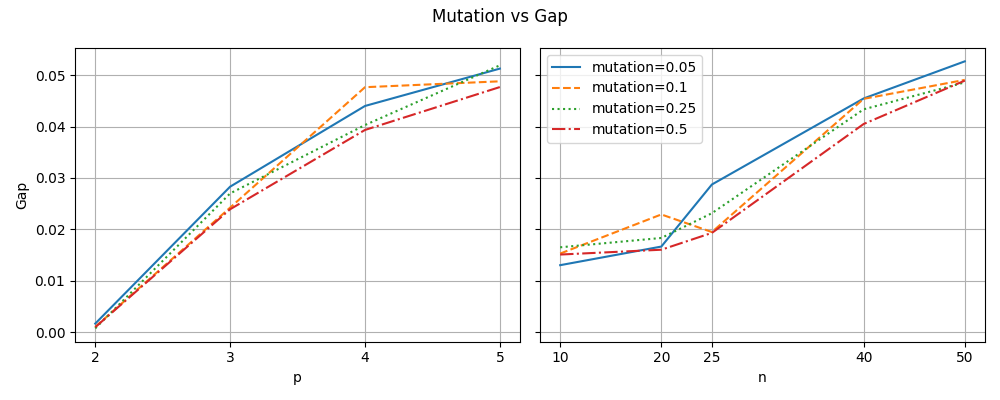
\includegraphics[width=0.9\textwidth]{figures/mutation_vs_gap.png}
  \caption{p vs. Gap and n vs. Gap based on the mutation probability}
  \label{fig:mutation_vs_gap}
\end{figure}

From this result we can see that overall the highest mutation probability ($0.5$) gets the results
closer to the optimal solution, except on the problems were either $n$ or $p$ are minimal. In these
cases the minimum mutation ($0.05$) comes on top for $n=10$ and all the mutation values get almost
the same gap for $p=2$. Outside of these minimal problems were the set of solutions is not big
enough to get an advantage from a diverse population, the lower mutation probability performs
significantly worse, specially as $n$ and $p$ increases.

\subsection{Performance searching the optimal solution\label{ss:benchmark_optimal}}

During this benchmark the algorithm was executed until the solution given by the examples
was matched. In order to attempt this multiple times with different parameters the benchmark attempts
to find the optimal solution with different combinations that will scale down in mutability and scale up
in evaluations and population, in this order.

This way the benchmark will broad the parameters of the execution in order to attempt to find the solution
if the previous combination didn't work. First, it attempts it lowering the mutation probability (using $0.5$,
$0.25$ and $0.1$ as possible values), then it attempts to allow a bigger number of maximum evaluations
($4096$, $16384$, $65536$, $262144$ and $1048576$) and finally using a bigger population ($10$, $20$, $25$,
$40$, $50$, $75$, $100$). Each advance in the number of evaluations resets the mutation to the first one,
and the same occurs when sizing up the population.

The executions that succeeded in finding the optimal can be seen in the Table \ref{tb:optimal_benchmark}.
The table shows the \emph{mutation} and \emph{population} used in the first optimal finding for that subproblem,
and it also records the number of \emph{evaluations} and the \emph{time} required in the successful 
execution, in addition to the \emph{total time} required adding the execution time of the previous attempts.
Every missing subproblem, like all those for sizes $40$ and $50$ aside of those with $p=2$, where not
resolved with the optimal solution in any of the $105$ different attempts.

\begin{table}
\caption{Results of optimal search benchmark}
\label{tb:optimal_benchmark}
\begin{center}
\begin{tabular}{|c|c|c|c|c|r|r|r|}
\hline
n & p & objective & mutation & population & evaluations & success time (ms) & total time (ms) \\
\hline
10 & 2 & 167493 & 0.50 & 10 & 182 & 3.044 & 3.044 \\
10 & 3 & 136008 & 0.50 & 10 & 1546 & 5.773 & 5.773 \\
10 & 4 & 112396 & 0.50 & 10 & 1269 & 2.851 & 2.851 \\
10 & 5 & 91105 & 0.50 & 10 & 896 & 2.013 & 2.013 \\
20 & 2 & 172817 & 0.50 & 10 & 361 & 1.409 & 1.409 \\
20 & 3 & 151533 & 0.50 & 20 & 2370 & 10.279 & 12350.606 \\
20 & 4 & 135625 & 0.50 & 10 & 11429 & 40.242 & 79.070 \\
20 & 5 & 123130 & 0.25 & 25 & 67998 & 303.726 & 31189.384 \\
25 & 2 & 175542 & 0.50 & 10 & 898 & 3.935 & 3.935 \\
25 & 3 & 155256 & 0.25 & 20 & 185100 & 805.702 & 17759.136 \\
25 & 4 & 139197 & 0.25 & 20 & 10588 & 48.033 & 15338.338 \\
25 & 5 & 123574 & 0.25 & 20 & 9380 & 42.249 & 15330.658 \\
40 & 2 & 177472 & 0.50 & 10 & 536 & 4.207 & 4.207 \\
50 & 2 & 178484 & 0.50 & 10 & 1033 & 10.694 & 10.694 \\
\hline
\end{tabular}
\end{center}
\end{table}


One of they key findings from this analysis was that only two of the subproblems resolved benefited from
the increment of evaluations over $65536$, with the $(20,5)$ barely using a couple thousand more evaluations.
This means that the current evaluation usually fails as it converges into a population no diverse enough
that fails to get closer to the optimal solution and the extra evaluations won't solve it.

A good solution for this could have been using a bigger population, specially as the problems with a
bigger $n$ will also have a lot more possible solutions. Relating the population to $n$ was followed in \ref{ss:benchmark_evaluations}.
In this case the scaling would end up reaching that value, and more, if required; but as we see only one
problem, $(20,3)$, scalated until $n=population$, with another one, the $(20,5)$, going above $n$. This
could be pointing the sweet post for $population$ below $n$,

